\documentclass[xcolor=x11names,compress]{beamer}
\usepackage{hyperref} 
\usepackage{mybeamer}
\usepackage{mystyle}
\usepackage{bm}
\usepackage{tikz}
\usepackage{adjustbox}
\usepackage{booktabs}       % professional-quality tables
\setbeamercovered{transparent}
\usetikzlibrary{calc,shapes,positioning}
\usetikzlibrary{arrows}
\usetikzlibrary{fit}
\newcommand{\midarrow}{\tikz \draw[-triangle 90] (0,0) -- +(.1,0);}
% set arrow type and size by tikz
% alternative to 'Straight Barb' can be 'Latex, Stealth, Computer Modern Rightarrow'.
\usetikzlibrary{arrows.meta}
\tikzset{>={Straight Barb[width=1.3mm,length=1.3mm]}}


\newcommand{\ubar}[1]{\mkern2mu\underline{\mkern-2mu #1\mkern-2mu}\mkern2mu}
\begin{document}


\begin{frame}
  \title{Approximate Inference and Learning: From Message-Passing to Neural Network based Methods}
  \subtitle{}
  % \includegraphics[height=1cm,width=2cm]{kth_eng_cmyk_wireless.eps}
  \author{ \small Dong Liu
    \\
    \vspace{0.3cm}
    % {\scriptsize with} {\small Ragnar Thobaben} {\scriptsize and} {\small Lars K. Rasmussen}
    \\
    \vspace{0.3cm}
    {\it \scriptsize Information Science and Engineering \\
      KTH - Royal Institute of Technology}
    % {\it $^2$ Department of Electrical Engineering, Princeton University.}
  }
  \vspace{-0.5cm}
  \date{
    \includegraphics[height=2cm,angle=0]{kth_eng_cmyk_wireless.eps}    
    \vspace{0.3cm}
    \scriptsize
    
    % Internal Seminar
  }
  \titlepage
\end{frame}

%%%%%%%%%%%%%%%%%%%%%%%%%%%%%%%%%%%%%%%%%%%%%%%%%%%%%% 
% ------------------------------------------------

%%%%%%%%%%%%%%%%%%%%%%%%%%%%%%%%%%%%%%%%%%%%%%%%%%%%%% 
\section{Content}
\subsection{Content}
\begin{frame}{\large Content}
  \begin{itemize}[label=$\bullet$]
  \item Background: Probabilistic graphical models (PGM)
  \item Common usage of PGMs
  \item High-level view of inference
  \item Play inference with neural networks
  \item Summary
  \end{itemize}
  
\end{frame}



% \begin{frame}{\large Content}
%   \begin{tikzpicture}
%     \tikzstyle{enode} = [thick, draw=black, ellipse, inner sep = 2pt,  align=center]
%     \node[enode] (fd) at (0,0) {Fundamental Problems};
%     \node[enode] (fd) at (0,-1) {General Methods};
%     \node[enode] (fd) at (0,-2) {Gibbs Simpling};
%     \node[enode] (fd) at (0,-3) {Mean Field};
%     \node[enode] (fd) at (0,-4) {Loopy Belief Propagation};
%     \node[enode] (fd) at (0,-5) {Generalized Belief Propagation};
%     \node[enode] (fd) at (0,-6) {Our approximation: RENN};
%     \node[enode] (fd) at (0,-7) {Application scenarios/examples};
%     \node[enode] (fd) at (0,-8) {Some numerical results};
%   \end{tikzpicture}

% \end{frame}


%%%%%%%%%%%%%%%%%%%%%%%%%%%%%%%%%%%%%%%%%%%%%%%%%%%%%% 
% ------------------------------------------------
\scriptsize
%%%%%%%%%%%%%%%%%%%%%%%%%%%%%%%%%%%%%%%%%%%%%%%%%%%%%% 
\section{PGM}
\scriptsize
\subsection{Probabilistic Graphical Models}
{ \setbeamercolor{background canvas}{bg=hl_bg}
  \setbeamercolor{normal text}{fg=hl_fg}
  \setbeamercolor{frametitle}{fg=hl_fg}
  \begin{frame}
    \usebeamercolor[fg]{normal text}
    \begin{center}
      {\large A few words on Probabilistic Graphical Models}
    \end{center}
    
  \end{frame}
}

\begin{frame}{Probabilistic Graphical Models}
  \begin{itemize}
    
    \item Directed: Bayesian Networks \\
      \vskip 0.2cm
      \begin{columns}
        \column{0.5\textwidth}
        \hskip 1cm
        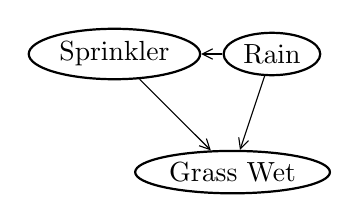
\begin{tikzpicture}
          % \tikzstyle{enode} = [thick, draw=blue, circle, inner sep = 3pt,
          % align=center]
          \tikzstyle{enode} = [thick, draw=black, ellipse, inner sep = 2pt,  align=center]
          \tikzstyle{nnode} = [thick, rectangle, rounded corners = 2pt, minimum size = 0.5cm,draw,inner sep = 2pt]

          \node[enode] (s) at (-0.5, 1.5) {Sprinkler};
          \node[enode] (r) at (1.5, 1.5) {Rain};
          \node[enode] (gw) at (1, 0) {Grass Wet};
          \draw[->] (r) to (s);
          \draw[->] (r) to (gw);
          \draw[->] (s) to (gw);
        \end{tikzpicture}

        \column{0.5\textwidth}
        \hskip -1cm
        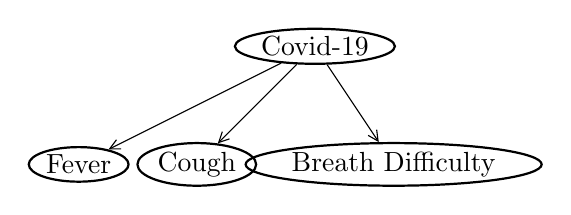
\begin{tikzpicture}
          \tikzstyle{cnode} = [thick, draw=black, ellipse, inner sep = 1pt,  align=center]
          \tikzstyle{nnode} = [thick, rectangle, rounded corners = 0pt,draw,inner sep = 2pt]
          \node[cnode] (virus) at (0, 1.5) {Covid-19};
          \node[cnode] (fever) at (-3, 0) {Fever};
          \node[cnode] (cough) at (-1.5, 0) {Cough};
          \node[cnode] (breath) at (1, 0) {Breath Difficulty};
          \draw[->] (virus) -- (fever);
          \draw[->] (virus) -- (cough);
          \draw[->] (virus) -- (breath);
        \end{tikzpicture}
        
      \end{columns}
    \item Undirected: Markov Random Field
      \vskip 0.2cm

      \begin{columns}
        \column{0.5\textwidth}
        \hskip 1cm
        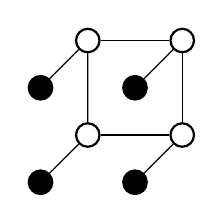
\begin{tikzpicture}[scale=0.6]
          \tikzstyle{enode} = [thick, draw, circle, inner sep = 3pt,  align=center]
          \tikzstyle{cnode} = [thick, fill=black, draw, circle, inner sep = 3pt,  align=center]
          \begin{scope}{scale=0.4, xshift=1cm}
            \node[enode] (x1) at (-2, 1) {};
            \node[enode] (x2) at (0, 1) {};
            \node[enode] (x3) at (-2, -1) {};
            \node[enode] (x4) at (0, -1) {};

            \node[cnode] (y1) at (-3, 0) {};
            \node[cnode] (y2) at (-1, 0) {};
            \node[cnode] (y3) at (-3, -2) {};
            \node[cnode] (y4) at (-1, -2) {};

            \draw[-] (x1) to (y1);
            \draw[-] (x2) to (y2);
            \draw[-] (x3) to (y3);
            \draw[-] (x4) to (y4);

            \draw[-] (x1) to (x2);
            \draw[-] (x1) to (x3);
            \draw[-] (x2) to (x4);
            \draw[-] (x3) to (x4);
          \end{scope}
        \end{tikzpicture}
        \vskip 0.1cm
        \hskip 1cm
        Computer vision
        \column{0.5\textwidth}
        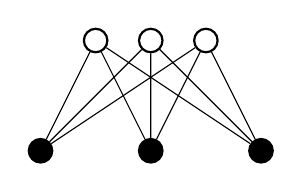
\begin{tikzpicture}[scale=0.7]
          \tikzstyle{enode} = [thick, draw, circle, inner sep = 3pt,  align=center]
          \tikzstyle{cnode} = [thick, fill=black, draw, circle, inner sep = 3pt,  align=center]
          \begin{scope}{scale=0.2}
            \node[enode] (x1) at (-2, 1) {};
            \node[enode] (x2) at (-1, 1) {};
            \node[enode] (x3) at (0, 1) {};

            \node[cnode] (y1) at (-3, -1) {};
            \node[cnode] (y2) at (-1, -1) {};
            \node[cnode] (y3) at (1, -1) {};
            

            \draw[-] (x1) to (y1);
            \draw[-] (x1) to (y2);
            \draw[-] (x1) to (y3);

            \draw[-] (x2) to (y1);
            \draw[-] (x2) to (y2);
            \draw[-] (x2) to (y3);

            \draw[-] (x3) to (y1);
            \draw[-] (x3) to (y2);
            \draw[-] (x3) to (y3);
            
            % \draw[-] (x4) to (y4);

            % \draw[-] (x1) to (x2);
            % \draw[-] (x1) to (x3);
            % \draw[-] (x2) to (x4);
            % \draw[-] (x3) to (x4);
          \end{scope}
        \end{tikzpicture}
        
        Communication system
      \end{columns}
    
  \end{itemize}
  Two key aspects to encode in a graphical model:

    \begin{itemize}[label={$\bullet$}]
    \item attributes of our interests in a system $\rightarrow$ variable nodes
    \item relationship of these factors (dependencies or indepedencies) $\rightarrow$ structures of a graph
    \end{itemize}
\end{frame}



\begin{frame}{\large Markov Random Field}
  \framesubtitle{Markov Random Field (MRF) and Fundamental Inference Problems}
  % \onslide<1->{
    
  % }
  \onslide<1->{
    Let us walk through via MRF
    \begin{itemize}[label={$\bullet$}]
    \item An MRF can be represented by a graph $\Gg(\Vv, \Ee)$ with each node $i\in \Vv$ is associated with a random variable $X_i$
    \item The probability distribution (Gibbs distribution) is
      \begin{equation*}\label{eq:joint-px}
        p(\bm{x}; \bm{\theta}) = \frac{1}{Z(\bm{\theta})} \prod_{a} \psi_a(\bm{x}_a; \bm{\theta}_a),
      \end{equation*}
      where $\bm{x}=\left\{ x_1, x_2, \cdots, x_N \right\}$, $a$ indexes potential functions $\Ii=\{\psi_A, \psi_B, \cdots, \psi_M\}$ and $\bm{\theta}$ is set of potential function parameters. $Z(\bm{\theta}) = \sum_{\bm{x}}\prod_{a} \psi_a(\bm{x}_a;\bm{\theta}_a)$.
    \end{itemize}
  }
  
\end{frame}


{ \setbeamercolor{background canvas}{bg=hl_bg}
  \setbeamercolor{normal text}{fg=hl_fg}
  \setbeamercolor{frametitle}{fg=hl_fg}
  \begin{frame}
    \usebeamercolor[fg]{normal text}
    \begin{center}
      {\large What do we do with graphical models?}
    \end{center}
    
  \end{frame}
}

\begin{frame}{Usage of Graphical Models}
  In general:
  \begin{itemize}[label={$\bullet$}]
    \onslide<1->{
    \item Representation\\
      \begin{itemize}[label={$\bullet$}]
      \item In place of real systems 
      \item Abstraction of complex problems or systems (with subjective bias)
      \end{itemize}
    \item Answer queries\\ Evidence (observation) $\rightarrow$ ?? $\rightarrow$ Answers}
    
  \end{itemize}
  \onslide<2->{
    Two components interacting with each other:
    \begin{figure}[!t]
      \centering
      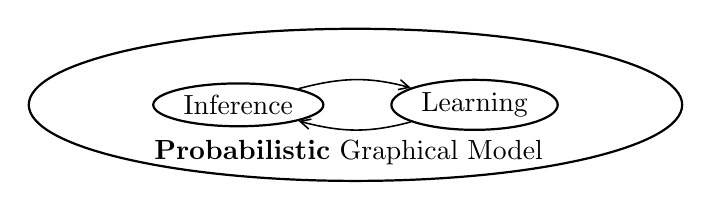
\begin{tikzpicture}
        \tikzstyle{cnode} = [thick, draw=black, ellipse, inner sep = 2pt,  align=center]
        \tikzstyle{fnode} = [thick, draw=black, ellipse, inner sep = 10pt,  align=center]
        
        \node[cnode] (infn) at (0,0) {Inference};
        \node[cnode] (lern) at (3,0) {Learning};
        
        \node[fnode, fit=(infn)(lern)] (box) {};
        \node[] at (1.4, -0.6) {\textbf{Probabilistic} Graphical Model};
        \draw[->,line width=0.2mm] (infn) to[out=15, in=165] (lern);
        \draw[->,line width=0.2mm] (lern) to[out=195, in=-15] (infn);
      \end{tikzpicture}
      
      \label{fig:intro-pgm}
    \end{figure}
  }
  
\end{frame}

\begin{frame}{Usage of Graphical Models}
  Why impact in two direction?


  \begin{itemize}[label=$\bullet$]
    \onslide<1>{
    \item Learning to Inference:\\
      \begin{figure}[!t]
        \centering
        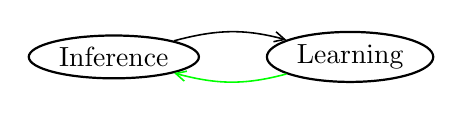
\begin{tikzpicture}
          \tikzstyle{cnode} = [thick, draw=black, ellipse, inner sep = 2pt,  align=center]
          \tikzstyle{fnode} = [thick, draw=black, ellipse, inner sep = 10pt,  align=center]
          
          \node[cnode] (infn) at (0,0) {Inference};
          \node[cnode] (lern) at (3,0) {Learning};
          
          % \node[fnode, fit=(infn)(lern)] (box) {};
          % \node[] at (1.4, -0.6) {Probabilistic Graphical Model};
          \draw[->,line width=0.2mm] (infn) to[out=15, in=165] (lern);
          \draw[green, ->,line width=0.2mm] (lern) to[out=195, in=-15] (infn);
        \end{tikzpicture}
      \end{figure}
      A graphical model
      \begin{itemize}[label=$\bullet$]
      \item built by expert knowledge, or
      \item built by extracting information from evidence (empirical data).
      \end{itemize}
      }
    \onslide<2->{
    \item Inference to Learning:\\
      \begin{figure}[!t]
        \centering
        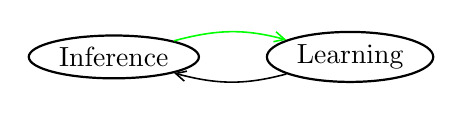
\begin{tikzpicture}
          \tikzstyle{cnode} = [thick, draw=black, ellipse, inner sep = 2pt,  align=center]
          \tikzstyle{fnode} = [thick, draw=black, ellipse, inner sep = 10pt,  align=center]
          
          \node[cnode] (infn) at (0,0) {Inference};
          \node[cnode] (lern) at (3,0) {Learning};
          
          % \node[fnode, fit=(infn)(lern)] (box) {};
          % \node[] at (1.4, -0.6) {Probabilistic Graphical Model};
          \draw[green, ->,line width=0.2mm] (infn) to[out=15, in=165] (lern);
          \draw[->,line width=0.2mm] (lern) to[out=195, in=-15] (infn);
        \end{tikzpicture}
      \end{figure}
      Model learning: an error trial process that compares inferred 'fact' and actual fact (evidence).\\
      Model learning usually needs inference as a subroutine, which sometimes are replaced by sampling in particle based methods.
    }
  \end{itemize}
  
  
\end{frame}


\begin{frame}{\large Common Inference Problems}
  The common inference problems in a MRF $\Gg(\Vv, \Ee)$:
  \begin{itemize}[label={$\bullet$}]
  \item Computing the likelihood of observed data.
  \item Computing the marginals distribution $p(\bm{x}_A)$ over particular subset $A \subset \Vv$ of nodes
  \item Computing the conditional distribution $p(\bm{x}_A | \bm{x}_{B})$, 
  \item Computing the most likely configuration $\argmax_{\bm{x}} p(\bm{x})$
  \end{itemize}
  \onslide<2>{
  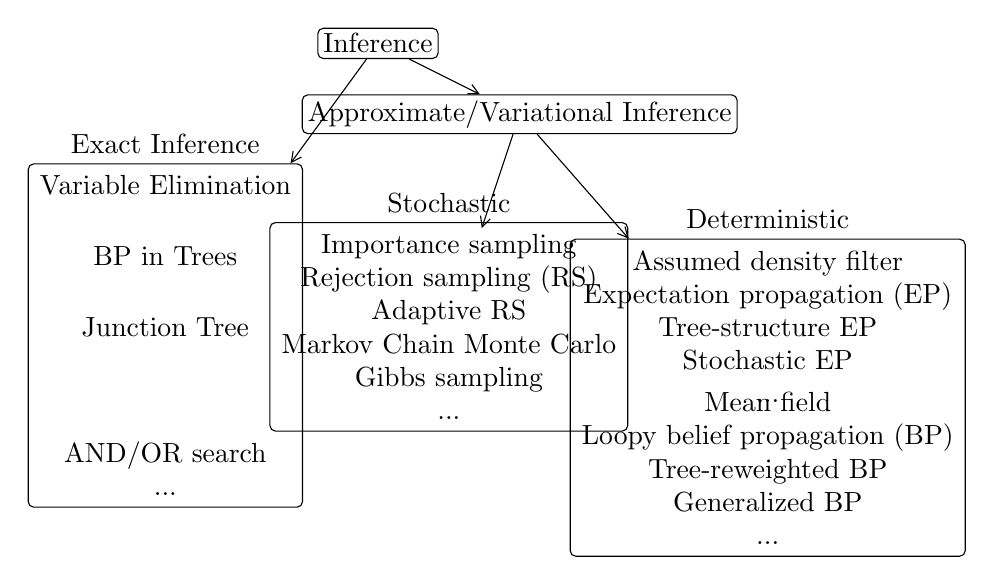
\begin{tikzpicture}[scale=0.9]
    \tikzstyle{nnode} = [rectangle, rounded corners=2pt, inner sep = 2pt,  align=center]
    \tikzstyle{rnode} = [draw=black, rectangle, rounded corners=2pt, inner sep = 2pt,  align=center]

    \node[rnode, opacity=1] (inf) at (0,0) {Inference};
    
    \node[rnode] (apx) at (2,-1) {Approximate/Variational Inference};

    \node[nnode] (e1) at (-3,-2) {Variable Elimination};
    \node[nnode] (e2) at (-3,-3) {BP in Trees};
    \node[nnode] (e3) at (-3,-4) {Junction Tree};
    \node[nnode] (e4) at (-3,-6) {AND/OR search\\ ...};

    \node[rnode, fit=(e1)(e2)(e3)(e4), label=above:{Exact Inference}] (exact) {};
    
    
    
    
    \node[nnode] (sto) at (1,-4) {
      Importance sampling\\
      Rejection sampling (RS) \\
      Adaptive RS \\
      Markov Chain Monte Carlo\\
      Gibbs sampling\\
      ...
    };
    \node[rnode, fit=(sto), label=above:{Stochastic}] {};

    \node[nnode] (d1) at (5.5,-6) {
      Mean field\\
      Loopy belief propagation (BP)  \\
      Tree-reweighted BP\\
      Generalized BP\\
      ...
    };
    \node[nnode] (d2) at (5.5,-4) {
      Assumed density filter \\
      Expectation propagation (EP)  \\
      Tree-structure EP\\
      Stochastic EP\\
      ...
    };

    \node[rnode, fit=(d1)(d2), label=above:{Deterministic}] (det) {};

    \draw[->] (inf) -- (exact);
    \draw[->] (inf) -- (apx);
    \draw[->] (apx) -- (sto);
    \draw[->] (apx) -- (det);

  \end{tikzpicture}
  }
  
  
\end{frame}

\begin{frame}{\large Inference Routine in Learning}
  \onslide<1->{
    What is $\bm{\theta}$ in $p(\bm{x}; \bm{\theta}) = \frac{1}{Z(\bm{\theta})} \prod_{a} \psi_a(\bm{x}_a; \bm{\theta}_a)$? \\
    A direct view:
    \begin{align*}
      \max_{\bm{\theta}} \log{p(\bm{x}; \bm{\theta})} =  \max_{\bm{\theta}}\sum_{a}\log{ \psi_a(\bm{x}_a; \bm{\theta}_a) } \underbrace{- \log{Z(\bm{\theta})}}_{Helmholtz~free~energy},
    \end{align*}
  }
  \onslide<2->{
    An alternative view:
    \begin{align*}
      \pd{\log{p}(\bm{x};\bm{\theta})}{\bm{\theta}_a} = \pd{\log{{\phi_a}(\bm{x}_a; \bm{\theta}_a)}}{\bm{\theta}_a} - \EE_{p(\bm{x}_a; \bm{\theta})}\left[ \pd{\log{{\phi_a}(\bm{x}_a; \bm{\theta}_a)}}{\bm{\theta}_a} \right].
    \end{align*}

    Remark:
    \begin{itemize}[label={$\bullet$}]
    \item This essentially requires estimation of Helmholtz free energy or marginal probabilities.
    \item Stationary points translate into moment matching.
    \end{itemize}
  }
\end{frame}


% \begin{frame}
%   \frametitle{A biased incomplete branching to methods}
%   \begin{tikzpicture}
%     \tikzstyle{nnode} = [rectangle, rounded corners=2pt, inner sep = 2pt,  align=center]
%     \tikzstyle{rnode} = [draw=black, rectangle, rounded corners=2pt, inner sep = 2pt,  align=center]

%     \node[rnode, opacity=1] (inf) at (0,0) {Inference};
    
%     \node[rnode] (apx) at (2,-1) {Approximate/Variational Inference};

%     \node[nnode] (e1) at (-3,-2) {Variable Elimination};
%     \node[nnode] (e2) at (-3,-3) {BP in Trees};
%     \node[nnode] (e3) at (-3,-4) {Junction Tree};
%     \node[nnode] (e4) at (-3,-6) {AND/OR search\\ ...};

%     \node[rnode, fit=(e1)(e2)(e3)(e4), label=above:{Exact Inference}] (exact) {};
    
    
    
    
%     \node[nnode] (sto) at (1,-4) {
%       Importance sampling\\
%       Rejection sampling (RS) \\
%       Adaptive RS \\
%       Markov Chain Monte Carlo\\
%       Gibbs sampling\\
%       ...
%     };
%     \node[rnode, fit=(sto), label=above:{Stochastic}] {};

%     \node[nnode] (d1) at (5,-6) {
%       Mean field\\
%       Loopy belief propagation (BP)  \\
%       Tree-reweighted BP\\
%       Generalized BP\\
%       ...
%     };
%     \node[nnode] (d2) at (5,-4) {
%       Assumed density filter \\
%       Expectation propagation (EP)  \\
%       Tree-structure EP\\
%       Stochastic EP\\
%       ...
%     };

%     \node[rnode, fit=(d1)(d2), label=above:{Deterministic}] (det) {};

%     \draw[->] (inf) -- (exact);
%     \draw[->] (inf) -- (apx);
%     \draw[->] (apx) -- (sto);
%     \draw[->] (apx) -- (det);

%   \end{tikzpicture}
  
% \end{frame}


%%%%%%%%%%%%%%%%%%%%%%%%%%%%%%%%%%%%%%%%%%%%%%%%%%%%%% 
% ------------------------------------------------
%%%%%%%%%%%%%%%%%%%%%%%%%%%%%%%%%%%%%%%%%%%%%%%%%%%%%% 
\section{Inference}
\subsection{Collection of Inference Methods}
{ \setbeamercolor{background canvas}{bg=hl_bg}
  \setbeamercolor{normal text}{fg=hl_fg}
  \setbeamercolor{frametitle}{fg=hl_fg}
  \begin{frame}
    \usebeamercolor[fg]{normal text}
    \begin{center}
      {\large
        Play with
        \textbf{Gibbs (variational) free energy}
        \begin{equation*}
          F_V(b) = \mathrm{KL}(b( \bm{x}) || p(\bm{x}; \bm{\theta})) - \log{Z(\bm{\theta})}
        \end{equation*}
        with trial $b(\bm{x})$.
      }
    \end{center}
    
  \end{frame}
}


\subsection{Intuition of Message Passing}
\begin{frame}{What is the state of $x$?}
  \framesubtitle{A toy example}
  Assume that we are interested into the state of node $i$ in an MRF, it can be answered by
  \begin{itemize}[label={$\bullet$}]
  \item the probability $p(x_i)$, or
  \item an empirical version, a collection of samples $\left\{ x_i^n \right\}_{n=1}^{N}$
  \end{itemize}
  It is similar for the case when $\bm{x}$ is of interests, instead of $x_i$.
  \begin{figure}
    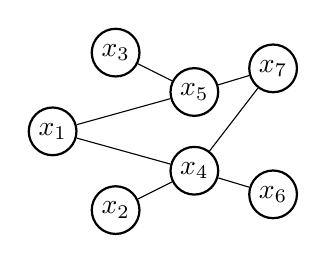
\begin{tikzpicture}
      % \tikzstyle{enode} = [thick, draw=blue, circle, inner sep = 3pt,
      % align=center]
      \tikzstyle{enode} = [thick, draw=black, circle, inner sep = 2pt,  align=center]
      \node[enode] (x1) at (-0.8,0) {$x_1$};
      \node[enode] (x2) at (0,-1) {$x_2$};
      \node[enode] (x3) at (0,1) {$x_3$};
      \node[enode] (x4) at (1,-0.5) {$x_4$};
      \node[enode] (x5) at (1,0.5) {$x_5$};
      \node[enode] (x6) at (2,-0.8) {$x_6$};
      \node[enode] (x7) at (2,+0.8) {$x_7$};

      \draw[-] (x1) to (x4);
      \draw[-] (x1) to (x5);
      \draw[-] (x2) to (x4);
      
      \draw[-] (x3) to (x5);
      \draw[-] (x4) to (x6);
      \draw[-] (x4) to (x7);
      \draw[-] (x5) to (x7);
    \end{tikzpicture}
    \captionsetup{labelformat=empty,justification=centering}
    \caption{what is the state of $x_4$}
    
  \end{figure}
  
\end{frame}

\begin{frame}{What is the state of $x$?}
  \framesubtitle{Gibbs sampling: let us guess by sampling}
  We can approximately sample iteratively: $  x_i \sim p(x_i|\bm{x}_{-i}) \sim p(x_i,\bm{x}_{-i})$
  \begin{figure}
    \begin{subfigure}{0.3\textwidth}
      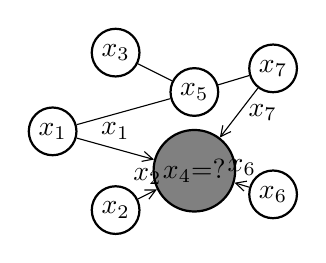
\begin{tikzpicture}
        % \tikzstyle{enode} = [thick, draw=blue, circle, inner sep = 3pt,
        % align=center]
        \tikzstyle{enode} = [thick, draw=black, circle, inner sep = 2pt,  align=center]
        \node[enode] (x1) at (-0.8,0) {$x_1$};
        \node[enode] (x2) at (0,-1) {$x_2$};
        \node[enode] (x3) at (0,1) {$x_3$};
        \node[enode, fill=gray] (x4) at (1,-0.5) {$x_4$=?};
        \node[enode] (x5) at (1,0.5) {$x_5$};
        \node[enode] (x6) at (2,-0.8) {$x_6$};
        \node[enode] (x7) at (2,+0.8) {$x_7$};

        \draw[->] (x1) to node[above] {$x_1$} (x4);
        \draw[-] (x1) to (x5);
        \draw[->] (x2) to node[above] {$x_2$} (x4);
        
        \draw[-] (x3) to (x5);
        \draw[->] (x6) to node[above] {$x_6$} (x4);
        \draw[->] (x7) to node[right] {$x_7$} (x4);
        \draw[-] (x5) to (x7);
      \end{tikzpicture}
      \captionsetup{labelformat=empty,justification=centering}
    \end{subfigure}
    \hskip 0.3in
    \begin{subfigure}{0.3\textwidth}
      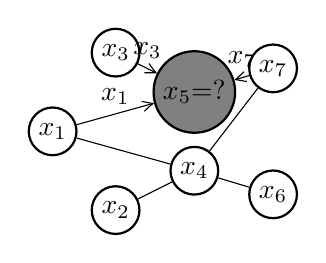
\begin{tikzpicture}
        \tikzstyle{enode} = [thick, draw=black, circle, inner sep = 2pt,  align=center]
        \node[enode] (x1) at (-0.8,0) {$x_1$};
        \node[enode] (x2) at (0,-1) {$x_2$};
        \node[enode] (x3) at (0,1) {$x_3$};
        \node[enode] (x4) at (1,-0.5) {$x_4$};
        \node[enode, fill=gray] (x5) at (1,0.5) {$x_5$=?};
        \node[enode] (x6) at (2,-0.8) {$x_6$};
        \node[enode] (x7) at (2,+0.8) {$x_7$};

        \draw[-] (x1) to (x4);
        \draw[->] (x1) to node[above] {$x_1$} (x5);
        \draw[-] (x2) to (x4);
        
        \draw[->] (x3) to node[above] {$x_3$} (x5);
        \draw[-] (x4) to (x6);
        \draw[-] (x4) to (x7);
        \draw[->] (x7) to node[above] {$x_7$} (x5);
      \end{tikzpicture}
      \captionsetup{labelformat=empty,justification=centering}
    \end{subfigure}
    
  \end{figure}
  This coordinate-wise sampling algorithm is called Gibbs sampling, which answers queries by collected samples $\left\{ \bm{x}^n \right\}_{1}^{N}$.
  \let\thefootnote\relax\footnotetext{\tiny Gibbs sampling is named after the physicist Josiah Willard Gibbs, which was described by brothers Stuart and Donald Geman in 1984, some eight decades after the death of Gibbs.\\
    \begin{equation*}
    x_i \sim \exp\{ \sum_{a \in \mathrm{ne}_i} \log{\phi_{a}}(x_i, \bm{x}_{a-i};\bm{\theta}_{a}) \}
  \end{equation*}
  where $\mathrm{ne}_i$ gives the neighboring potential factors of node $i$.
  }
\end{frame}

\begin{frame}{What is the state of $x$?}
  Naive Mean Field: \textbf{message in form of sample values $\rightarrow$ message in form of belief}
  \begin{figure}
    
    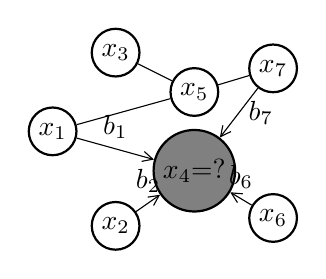
\begin{tikzpicture}
      \tikzstyle{enode} = [thick, draw=black, circle, inner sep = 2pt,  align=center]
      \node[enode] (x1) at (-0.8,0) {$x_1$};
      \node[enode] (x2) at (0,-1.2) {$x_2$};
      \node[enode] (x3) at (0,1) {$x_3$};
      \node[enode, fill=gray] (x4) at (1,-0.5) {$x_4$=?};
      \node[enode] (x5) at (1,0.5) {$x_5$};
      \node[enode] (x6) at (2,-1.1) {$x_6$};
      \node[enode] (x7) at (2,+0.8) {$x_7$};

      \draw[->] (x1) to node[above=0.05mm] {$b_1$} (x4);
      \draw[-] (x1) to (x5);
      \draw[->] (x2) to node[above=0.05mm] {$b_2$}(x4);
      
      \draw[-] (x3) to (x5);
      \draw[->] (x6) to node[above=0.05mm] {$b_6$} (x4);
      \draw[->] (x7) to node[right] {$b_7$} (x4);
      \draw[-] (x5) to (x7);
    \end{tikzpicture}
  \end{figure}
  Corresponding to minimization of \textbf{variational free energy $F_v(b)$  with trial $b$ in fully-factorized form for univariant $\{b_i\}$}.
  \let\thefootnote\relax\footnotetext{\tiny
    Iterative sampling $\rightarrow$ iterative belief update via  
    \begin{equation*}
      \log{b_i(x_i)} \propto \sum_{a \in \mathrm{ne}_i} \sum_{\bm{x}_{a} \backslash x_i} \prod_{j\in {a}\backslash i} b_j(x_j)\log{\phi_{a}}(\bm{x}_{a};\bm{\theta}_{a}).
    \end{equation*}  
  }
\end{frame}

\begin{frame}{What is the state of $x$?}
  \framesubtitle{Belief propagation (BP): let us guess by propagating belief}
  \onslide<1->{

    Proposed by Pearl (1982) for Bayesian networks (tree-structured graphs), which then widely used for general graphs (loopy BP).
    
    {Yedidia, et al, connected the loopy BP with stationary points of \textbf{Bethe free energy}
      \begin{align*}
        F_{Bethe}(b) = \sum_{a\in \Ff} \sum_{\bm{x}_{a}}
        b_{a}(\bm{x}_{a})\log{\frac{b_{a}(\bm{x}_{a})}{\phi_{a}(\bm{x}_{a})}
        } -  \sum_{i=1}^{N} (|\mathrm{ne}_i| - 1) \sum_{x_i} b_i(x_i) \log{b_i(x_i)},
      \end{align*}
    }
    
    Corresponding to minimization of approximated \textbf{variational free energy $F_v(b)$  with trial $b$ includes $\{b_i\}$ and $\{b_a\}$}.

    }
    \let\thefootnote\relax\footnotetext{\tiny
      \vskip -0.8cm
      \begin{align*}
    \mathrm{msg: factor~ to~ variable} ~~ m_{a\rightarrow i}(x_i) & \propto \sum_{\bm{x}_{a} \backslash x_i}
                                \phi_{a}(\bm{x}_{a}) \prod_{j \in a \backslash i} m_{j\rightarrow a}(x_j), \\
    \mathrm{msg: variable~ to~ factor} ~~  m_{j\rightarrow a}(x_j) & \propto  \prod_{a^{\prime} \in \mathrm{ne}_j
                                \backslash a} m_{a^{\prime}\rightarrow j}(x_j)
    \end{align*}
    See, D. Liu, M. T. Vu, Z. Li, and Lars K. Rasmussen. $\alpha$ belief propagation for approximate inference. 2020 \\
    D. Liu, N. N. Moghadam, L. K. Rasmussen, etc. $\alpha$ belief propagation as fully factorized approximation. In
    GlobalSIP, 2019.
    for alternative view to loopy BP.
  }
  
\end{frame}


\begin{frame}{What is the state of $x$?}
  \framesubtitle{Yedidia, Freeman, Weiss: A step to generalization}
  \textbf{Message among variables \& factors $\rightarrow$ message among regions}
  \vskip -0.5cm
  \begin{figure}
    \centering
    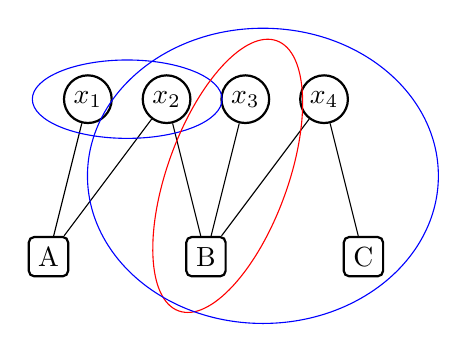
\begin{tikzpicture}
      % \tikzstyle{enode} = [thick, draw=blue, circle, inner sep = 3pt,
      % align=center]
      \tikzstyle{enode} = [thick, draw=black, circle, inner sep = 2pt,  align=center]
      \tikzstyle{nnode} = [thick, rectangle, rounded corners = 2pt, minimum size = 0.5cm,draw,inner sep = 2pt]
      \tikzstyle{fnode} = [draw=blue, ellipse, inner sep = 1pt]
      \tikzstyle{fnoder} = [draw=red, ellipse, inner sep = 0.0pt, rotate=-20]


      \node[enode] (x1) at (-1.5, 1) {$x_1$};
      \node[enode] (x2) at (-0.5, 1) {$x_2$};
      \node[enode] (x3) at (0.5, 1) {$x_3$};
      \node[enode] (x4) at (1.5, 1) {$x_4$};

      \node[nnode] (a) at (-2,-1) {A};
      \node[nnode] (b) at (0,-1) {B};
      \node[nnode] (c) at (2,-1) {C};

      \draw[-] (a) to (x1);
      \draw[-] (a) to (x2);
      \draw[-] (b) to (x2);
      \draw[-] (b) to (x3);
      \draw[-] (b) to (x4);
      \draw[-] (c) to (x4);
      
      \node[fnode, fit=(x1)(x2)] (box) {};
      \node[fnoder, fit=(x3)(b)] (box) {};

      \node[fnode, fit=(x2)(x3)(x4)(b)(c)] (box) {};
    \end{tikzpicture}
  \end{figure}
  \vskip -0.5cm
  
  % A region in a region graph acts as a node, and there are directed edges between regions which are defined according to specific rules. Formally, a region graph is defined as follows:

  % A \textit{region graph} is  a directed graph $\Gg_R(\Rr, \Ee)$, where each vertex $R \in \Rr$ is defined as the joint set of variable and factor nodes in this region, i.e., $R = \left\{ i \in V_R, a \in A_R | i \in \Vv, a \in \Ff \right\}$. Each edge $e \in \Ee$ in $\Gg_R$ is directed from $R_p$ to $R_c$ such that $R_c \subset R_p$. 

  Generalized belief propagation (GBP) generalizes loopy BP
  \begin{itemize}[label={$\bullet$}]
  \item usual better approximation than LBP
  \item higher complexity
  \item sensitive to scheduling of region messages
  \end{itemize}
  Corresponding to minimization of approximated \textbf{variational free energy $F_v(b)$  with trial $b$ including $\{b_R\}$}.
  \let\thefootnote\relax\footnotetext{\tiny
    \vskip -0.2cm
    A \textit{region} $R$ is a set $V_R$ of variables nodes and a set $A_R$ of factor nodes, such that if a factor node '$a$' belongs to $A_R$, all the variables nodes neighboring $a$ are in $V_R$.
}
\end{frame}
%%%%%%%%%%%%%%%%%%%%%%%%%%%%%%%%%%%%%%%%%%%%%%%%%%%%%% 
% ------------------------------------------------

%%%%%%%%%%%%%%%%%%%%%%%%%%%%%%%%%%%%%%%%%%%%%%%%%%%%%% 
\section{Inference with NNs}

{ \setbeamercolor{background canvas}{bg=hl_bg}
  \setbeamercolor{normal text}{fg=hl_fg}
  \setbeamercolor{frametitle}{fg=hl_fg}
  \begin{frame}
    \usebeamercolor[fg]{normal text}
    \begin{center}
      {\large Attempts with neural networks: an imitation game of message passing, or trials under free energy?}
    \end{center}
    
  \end{frame}
}
\subsection{GraphNet}

\begin{frame}{Learn the message update rule by NN}
  An end-to-end learning process: Factor graph $\rightarrow$ converted graph representation $\rightarrow$ GNN $\rightarrow$ Output
  \begin{figure}
    \centerline{\includegraphics[scale=0.3]{figures/gnn.png}}
  \end{figure}
  \begin{itemize}[label=$\bullet$]
  \item sum-product update rule (in BP) $\rightarrow$ NN, to learn
  \item pseudo probability (belief aggregation) $\rightarrow$ NN, to learn
  \item end-to-end learning that requires true marginal probability, which BP, GPB and mean field do no require
  \end{itemize}
  \let\thefootnote\relax\footnotetext{\tiny For related methods, see:\\
    Heess et al, Learning to Pass Expectation Propagation Messages\\
    Yoon, et al, 2019, Inference in Probabilistic Graphical Models by Graph Neural Networks\\
    Gilmer, et al, 2017, Neural message passing for quantum chemistry.\\
    Battaglia, et al, 2018, Relational inductive biases, deep learning, and graph networks
  }
\end{frame}

\subsection{AutoEncoder}

% \begin{frame}
%   {Variational Auto-encoder}
%   \onslide<1->{
%     \begin{itemize}[label=$\bullet$]
%     \item Simplification on structures \\
%       \begin{tikzpicture}
%         \tikzstyle{enode} = [thick, draw=black, circle, inner sep = 2pt,  align=center]
%         \tikzstyle{nnode} = [thick, rectangle, rounded corners = 2pt, minimum size = 0.5cm,draw,inner sep = 2pt]
%         \tikzstyle{fnode} = [draw=blue, ellipse, inner sep = 1pt]
%         \tikzstyle{fnoder} = [draw=red, ellipse, inner sep = 0.0pt, rotate=-20]

%         \begin{scope}[scale=0.5]
%           \node[enode] (x1) at (-1.5, 1) {$x_1$};
%           \node[enode] (x2) at (-1.5, -1) {$x_2$};
%           \node[enode] (x3) at (0.5, 1) {$x_3$};
%           \node[enode] (x4) at (0.5, -1) {$x_4$};
%           \draw (x1) -- (x2)
%           (x1) -- (x3)
%           (x4) -- (x3)
%           (x4) -- (x2)
%           ;
%         \end{scope}
%         \begin{scope}[scale=0.5, xshift=5cm]
%           \node[enode] (x1) at (-1.5, 1) {$x_1$};
%           \node[enode] (x2) at (-1.5, -1) {$x_2$};
%           \node[enode] (x3) at (0.5, 1) {$x_3$};
%           \node[enode] (x4) at (0.5, -1) {$x_4$};
%         \end{scope}

%       \end{tikzpicture}
%     }
%     \onslide<2->{
%     \item Care about only a certain set of variables \\
%       \begin{tikzpicture}
%         \tikzstyle{enode} = [thick, draw=black, circle, inner sep = 2pt,  align=center]
%         \tikzstyle{nnode} = [thick, rectangle, rounded corners = 2pt, minimum size = 0.5cm,draw,inner sep = 2pt]
%         \tikzstyle{fnode} = [draw=blue, ellipse, inner sep = 3pt]
        

%         \begin{scope}[scale=0.5]
%           \node[enode] (x1) at (-1.5, 1) {$x_1$};
%           \node[enode] (x2) at (-1.5, -1) {$x_2$};
%           \node[fnode, fit=(x1)(x2)] (xo){$\bm{x}_O$};
%         \end{scope}
%         \begin{scope}[scale=0.5, xshift=5cm]
%           \node[enode] (x3) at (0.5, 1) {$x_3$};
%           \node[enode] (x4) at (0.5, -1) {$x_4$};
%           \node[fnode, fit=(x3)(x4)] (xu) {$\bm{x}_U$};
%         \end{scope}

%       \end{tikzpicture}
%     }
%     \onslide<3->{
%     \item Amortizing the probabilities of interests and learn their parameters by sampling
%       \begin{tikzpicture}
%         \tikzstyle{enode} = [thick, draw=black, circle, inner sep = 2pt,  align=center]
%         \tikzstyle{nnode} = [thick, rectangle, rounded corners = 2pt, minimum size = 0.5cm,draw,inner sep = 2pt]
%         \tikzstyle{fnode} = [draw=blue, ellipse, inner sep = 3pt]
        
%         \node[fnode] (xo) at (0,0){$\bm{x}_O$};
%         \node[fnode] (xu) at (3,0) {$\bm{x}_U$};
%         \node[fnode] (hxo) at (6,0){$\hat{\bm{x}}_O$};
%         \draw[->] (xo) to node[above]{$q(\bm{x}_U|\bm{x}_O)$} (xu);
%         \draw[->](xu) to node[above]{${{p}(\bm{x}_O| \bm{x}_U; \bm{\theta})}$}(hxo);
%       \end{tikzpicture}
      
%       with the \textbf{variational free energy $F_V$ rewritten as}
%       \begin{equation*}
%         F_V(q, \bm{\theta}) = \EE_{q(\bm{x}_U|\bm{x}_O)}\left[ \log{{p}(\bm{x}_O| \bm{x}_U; \bm{\theta})} + \log{{p}(\bm{x}_U; \bm{\theta})} \right] + H({q(\bm{x}_U|\bm{x}_O)}),
%       \end{equation*}
%     }
%   \end{itemize}
% \end{frame}
\subsection{RENN}


\begin{frame}{RENN}
  \framesubtitle{Region revisited}
  \begin{itemize}[label=$\bullet$]
  \item If you cannot collect true targets ($p(x_i)$)
  \item If you are unwilling to be restricted to pre-defined inference  
  \end{itemize}
  \onslide<1->{
    Factor graph representation of MRF (2-by-3 grid) with factor nodes.\\
    MRF $\rightarrow$ region graph:\\
    \begin{columns}
      \column{0.5\textwidth}
      \hskip 1cm
      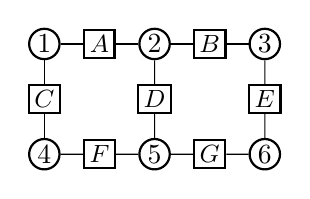
\begin{tikzpicture}
        \begin{scope}[scale=0.7]

          \tikzstyle{cnode} = [thick, draw=black, circle, inner sep = 1pt,  align=center]
          \tikzstyle{nnode} = [thick, rectangle, rounded corners = 0pt,draw,inner sep = 2pt]
          \node[cnode] (x1) at (0,0) {1};
          \node[cnode] (x2) at (2,0) {2};
          \node[cnode] (x3) at (4,0) {3};

          \node[cnode] (x4) at (0,-2) {4};
          \node[cnode] (x5) at (2,-2) {5};
          \node[cnode] (x6) at (4,-2) {6};

          \node[nnode] (fa) at (1,0) {\small$A$};
          \node[nnode] (fb) at (3,0) {\small$B$};

          \node[nnode] (fc) at (0,-1) {\small$C$};
          \node[nnode] (fd) at (2,-1) {\small$D$};
          \node[nnode] (fe) at (4,-1) {\small$E$};
          
          \node[nnode] (ff) at (1,-2) {\small$F$};
          \node[nnode] (fg) at (3,-2) {\small$G$};


          \draw[-] (x1) -- (fa);
          \draw[-] (x1) -- (fc);

          \draw[-] (x2) -- (fa);
          \draw[-] (x2) -- (fb);
          \draw[-] (x2) -- (fd);

          \draw[-] (x3) -- (fb);
          \draw[-] (x3) -- (fe);

          \draw[-] (x4) -- (fc);
          \draw[-] (x4) -- (ff);

          \draw[-] (x5) -- (fd);
          \draw[-] (x5) -- (ff);
          \draw[-] (x5) -- (fg);

          \draw[-] (x6) -- (fe);
          \draw[-] (x6) -- (fg);

        \end{scope}
      \end{tikzpicture}
    }
    \onslide<2->{
      \column{0.5\textwidth}

      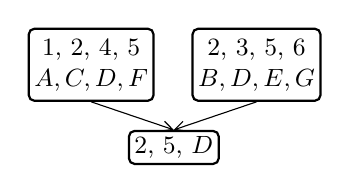
\begin{tikzpicture}
        \tikzstyle{cnode} = [thick, draw=black, circle, inner sep = 1pt,  align=center]
        \tikzstyle{nnode} = [thick, rectangle, rounded corners = 0pt,draw,inner sep = 2pt]

        \begin{scope}[xshift=4.8cm, yshift=-0.3cm,scale=0.7]
          \tikzstyle{rnode} = [thick, rectangle, rounded corners = 2pt,minimum size = 0.0cm,draw,inner sep = 2pt]
          \node[rnode] (r01) at (0,0) {\small \begin{tabular}[x]{@{}c@{}}1, 2, 4, 5 \\ $A,C,D,F$ \end{tabular}};
          \node[rnode] (r02) at (3,0) {\small \begin{tabular}[x]{@{}c@{}}2, 3, 5, 6\\ $B,D,E,G$ \end{tabular}};
          \node[rnode] (r11) at (1.5, -1.5) {\small 2, 5, $D$};

          \draw[->] (r01.south) -- (r11.north);
          \draw[->] (r02.south) -- (r11.north);

        \end{scope}
      \end{tikzpicture}

    \end{columns}
  % }
  % \onslide<3->{
    An alternative region graph of the same MRF:\\
    \centering
    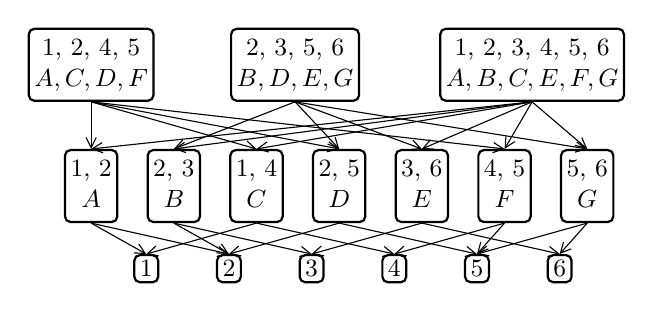
\begin{tikzpicture}
      \tikzstyle{cnode} = [thick, draw=black, circle, inner sep = 1pt,  align=center]
      \tikzstyle{nnode} = [thick, rectangle, rounded corners = 0pt,draw,inner sep = 2pt]

      \begin{scope}[xshift=0.6cm, yshift=-2.35cm,scale=0.7]
        \tikzstyle{rnode} = [thick, rectangle, rounded corners = 2pt,minimum size = 0.0cm,draw,inner sep = 2pt]
        \node[rnode] (r01) at (0,0) {\small\begin{tabular}[x]{@{}c@{}}1, 2, 4, 5 \\ $A,C,D,F$ \end{tabular}};
        \node[rnode] (r02) at (3.7,0) {\small\begin{tabular}[x]{@{}c@{}}2, 3, 5, 6\\ $B,D,E,G$ \end{tabular}};
        \node[rnode] (r03) at (8,0) {\small\begin{tabular}[x]{@{}c@{}}1, 2, 3, 4, 5, 6\\ $A,B,C,E,F,G$ \end{tabular}};
        \begin{scope}[yshift=-0.2cm]
          \node[rnode] (r11) at (0, -2.0) {\small\begin{tabular}[x]{@{}c@{}}1, 2\\ $A$ \end{tabular}};
          \node[rnode] (r12) at (1.5, -2.0) {\small\begin{tabular}[x]{@{}c@{}}2, 3\\ $B$ \end{tabular}};
          \node[rnode] (r13) at (3, -2.0) {\small\begin{tabular}[x]{@{}c@{}}1, 4\\ $C$ \end{tabular}};
          \node[rnode] (r14) at (4.5, -2.0) {\small\begin{tabular}[x]{@{}c@{}}2, 5\\ $D$ \end{tabular}};
          \node[rnode] (r15) at (6, -2.0) {\small\begin{tabular}[x]{@{}c@{}}3, 6\\ $E$ \end{tabular}};
          \node[rnode] (r16) at (7.5, -2.0) {\small\begin{tabular}[x]{@{}c@{}}4, 5\\ $F$ \end{tabular}};
          \node[rnode] (r17) at (9, -2.0) {\small\begin{tabular}[x]{@{}c@{}}5, 6\\ $G$ \end{tabular}};

          \begin{scope}[yshift=0.5cm]
            \node[rnode] (r21) at (1, -4) {\small 1};
            \node[rnode] (r22) at (2.5, -4) {\small 2};
            \node[rnode] (r23) at (4, -4) {\small 3};
            \node[rnode] (r24) at (5.5, -4) {\small 4};
            \node[rnode] (r25) at (7, -4) {\small 5};
            \node[rnode] (r26) at (8.5, -4) {\small 6};
          \end{scope}
        \end{scope}
        % edge level0 to level1
        \draw[->] (r01.south) -- (r11.north);
        \draw[->] (r03.south) -- (r11.north);

        \draw[->] (r02.south) -- (r12.north);
        \draw[->] (r03.south) -- (r12.north);

        \draw[->] (r01.south) -- (r13.north);
        \draw[->] (r03.south) -- (r13.north);

        \draw[->] (r01.south) -- (r14.north);
        \draw[->] (r02.south) -- (r14.north);

        \draw[->] (r02.south) -- (r15.north);
        \draw[->] (r03.south) -- (r15.north);

        \draw[->] (r01.south) -- (r16.north);
        \draw[->] (r03.south) -- (r16.north);

        \draw[->] (r02.south) -- (r17.north);
        \draw[->] (r03.south) -- (r17.north);

        % edge level1 to level2
        \draw[->] (r11.south) -- (r21.north);
        \draw[->] (r13.south) -- (r21.north);

        \draw[->] (r11.south) -- (r22.north);
        \draw[->] (r12.south) -- (r22.north);
        \draw[->] (r14.south) -- (r22.north);


        \draw[->] (r12.south) -- (r23.north);
        \draw[->] (r15.south) -- (r23.north);

        \draw[->] (r13.south) -- (r24.north);
        \draw[->] (r16.south) -- (r24.north);

        \draw[->] (r14.south) -- (r25.north);
        \draw[->] (r16.south) -- (r25.north);
        \draw[->] (r17.south) -- (r25.north);

        \draw[->] (r15.south) -- (r26.north);
        \draw[->] (r17.south) -- (r26.north);
      \end{scope}
    \end{tikzpicture}
  }
\end{frame}
\begin{frame}{RENN}
  \onslide<1->{
    The region-based free energy of a region graph is
    \begin{equation*}
      F_R(\Bb; \bm{\theta}) = \sum_{R\in \Rr} \underbrace{c_R}_{counting~number} \sum_{\bm{x}_R}b_R(\bm{x}_R) (\underbrace{E_R(\bm{x}_R; \bm{\theta}_R)}_{region~average~energy} + \ln{b_R}(\bm{x}_R)),
    \end{equation*}
    \begin{itemize}[label=$\bullet$]
    \item counting number: balance the contribution of each region
    \item region average energy: $- \sum_{a\in A_R} \ln{\phi_a(\bm{x}_a; \bm{\theta}_a)}$
    \end{itemize}
  }
  \onslide<2->{
    \begin{columns}
      \column{0.05\textwidth}
      Denote
      \column{0.3\textwidth}
      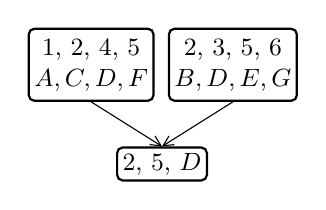
\begin{tikzpicture}
        \tikzstyle{cnode} = [thick, draw=black, circle, inner sep = 1pt,  align=center]
        \tikzstyle{nnode} = [thick, rectangle, rounded corners = 0pt,draw,inner sep = 2pt]
        
        \begin{scope}[xshift=0cm, yshift=-2.3cm,scale=0.6]
          \tikzstyle{rnode} = [thick, rectangle, rounded corners = 2pt,minimum size = 0.0cm,draw,inner sep = 2pt]
          \node[rnode] (r01) at (0,0) {\small \begin{tabular}[x]{@{}c@{}}1, 2, 4, 5 \\ $A,C,D,F$ \end{tabular}};
          \node[rnode] (r02) at (3,0) {\small \begin{tabular}[x]{@{}c@{}}2, 3, 5, 6\\ $B,D,E,G$ \end{tabular}};
          \node[rnode] (r11) at (1.5, -2.1) {\small 2, 5, $D$};

          \draw[->] (r01.south) -- (r11.north);
          \draw[->] (r02.south) -- (r11.north);

        \end{scope}
      \end{tikzpicture}
      \column{0.05\textwidth}
      by
      \column{0.3\textwidth}

      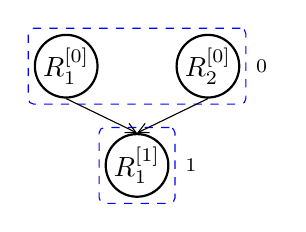
\begin{tikzpicture}
        \tikzstyle{cnode} = [thick, draw=black, circle, inner sep = 1pt,  align=center]
        \tikzstyle{nnode} = [dashed, draw=blue, rectangle, rounded corners = 2pt, inner sep = 2pt]
        
        \begin{scope}[xshift=0cm, yshift=2.3cm,scale=0.6]
          \tikzstyle{rnode} = [thick, circle, rounded corners = 2pt,minimum size = 0.0cm,draw,inner sep = 0.5pt]
          \node[rnode] (r01) at (0,0) {$R_1^{[0]}$};
          \node[rnode] (r02) at (3,0) {$R_2^{[0]}$};
          \node[rnode] (r11) at (1.5, -2.1) {$R_1^{[1]}$};
          \node[nnode, fit=(r01)(r02), label=right:$\Rr_0$] {};
          \node[nnode, fit=(r11), label=right:$\Rr_1$] {};

          \draw[->] (r01.south) -- (r11.north);
          \draw[->] (r02.south) -- (r11.north);

        \end{scope}
      \end{tikzpicture}
    \end{columns}
  }
  \onslide<3->{
    \begin{columns}
      \column{0.1\textwidth}
      Amortizing root beliefs:
      \column{0.7\textwidth}

      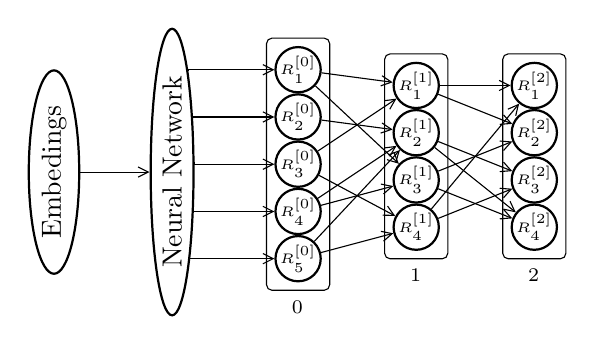
\begin{tikzpicture}
        
        \tikzstyle{enode} = [thick, draw=black, ellipse, inner sep = 2pt,  align=center]
        \tikzstyle{cnode} = [thick, draw=black, circle, inner sep = 0.0pt,  align=center]
        \tikzstyle{nnode} = [thick, rectangle, rounded corners = 0pt,draw,inner sep = 2pt]
        \begin{scope}[xshift=-1cm, yshift=-1.3cm, scale=0.6]
          \node[enode, rotate=90] (em) at (-2.5,0) {Embedings};
          \node[enode, rotate=90] (nn) {Neural Network};
        \end{scope}
        
        % level0 regions
        \begin{scope}[scale=0.6]
          \node[cnode] (r01) at (1, 0) {\tiny$R_1^{[0]}$};
          \node[cnode] (r02) at (1, -1) {\tiny$R_2^{[0]}$};
          \node[cnode] (r03) at (1, -2) {\tiny$R_3^{[0]}$};
          \node[cnode] (r04) at (1, -3) {\tiny$R_4^{[0]}$};
          \node[cnode] (r05) at (1, -4) {\tiny$R_5^{[0]}$};
          \node[label=below:$\Rr_0$, draw,rounded corners = 2pt, inner sep=1mm, fit=(r01) (r05)] {};
        \end{scope}

        \draw[->] (nn.351.9) |- (r01);
        \draw[->] (nn.340) |- (r02);
        \draw[->] (nn.295) |- (r03);
        \draw[->] (nn.210) |- (r04);
        \draw[->] (nn.191) |- (r05);

        \draw[->] (em) -- (nn);


        % level 1 regions
        \begin{scope}[xshift=1.5cm, yshift=-0.2cm, scale=0.6]
          \node[cnode] (r11) at (1, 0) {\tiny$R_1^{[1]}$};
          \node[cnode] (r12) at (1, -1) {\tiny$R_2^{[1]}$};
          \node[cnode] (r13) at (1, -2) {\tiny$R_3^{[1]}$};
          \node[cnode] (r14) at (1, -3) {\tiny$R_4^{[1]}$};
          \node[label=below:$\Rr_1$, draw, rounded corners = 2pt, inner sep=1mm, fit=(r11) (r14)] {};
        \end{scope}

        
        
        % level 1 regions
        \begin{scope}[xshift=3cm, yshift=-0.2cm, scale=0.6]
          \node[cnode] (r21) at (1, 0) {\tiny$R_1^{[2]}$};
          \node[cnode] (r22) at (1, -1) {\tiny$R_2^{[2]}$};
          \node[cnode] (r23) at (1, -2) {\tiny$R_3^{[2]}$};
          \node[cnode] (r24) at (1, -3) {\tiny$R_4^{[2]}$};
          \node[label=below:$\Rr_2$, draw, rounded corners = 2pt, inner sep=1mm, fit=(r21) (r24)] {};
        \end{scope}

        \draw[->] (r01) -- (r11);
        \draw[->] (r03) -- (r11);

        \draw[->] (r02) -- (r12);
        \draw[->] (r04) -- (r12);
        \draw[->] (r05) -- (r12);

        \draw[->] (r01) -- (r13);
        \draw[->] (r04) -- (r13);

        \draw[->] (r03) -- (r14);
        \draw[->] (r05) -- (r14);


        \draw[->] (r11) -- (r21);
        \draw[->] (r14) -- (r21);

        \draw[->] (r11) -- (r22);
        \draw[->] (r13) -- (r22);

        \draw[->] (r12) -- (r23);
        \draw[->] (r14) -- (r23);

        \draw[->] (r12) -- (r24);
        \draw[->] (r13) -- (r24);

        
        
      \end{tikzpicture}
    \end{columns}
  }
\end{frame}

\begin{frame}{RENN}
  \onslide<1->{
    Objective of RENN\footnote{\tiny More detail on RENN? Refer to, Dong Liu, Ragnar Thobaben, and Lars K. Rasmussen. Region-based energy
      neural network for approximate inference. arxiv, 2020}:\\
    \begin{equation*}
      \min \mathrm{\textbf{region-based free energy}} (F_R) + \underbrace{\mathrm{\textbf{panelty on belief consistency} }}_{along~ region~ graph~ struture}
    \end{equation*}
  }
  \\
  \onslide<2->{
    Inference only\\
    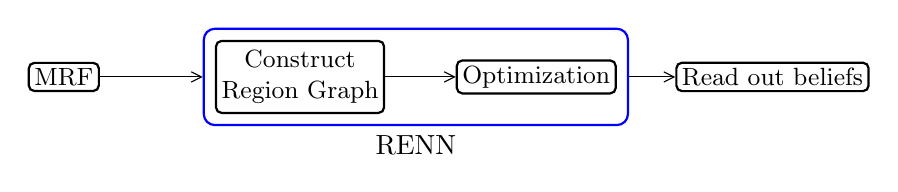
\begin{tikzpicture}
      \tikzstyle{cnode} = [thick, draw=blue, rounded corners = 4pt, rectangle, inner sep = 4pt,  align=center]
      \tikzstyle{nnode} = [thick, rectangle, rounded corners = 0pt,draw,inner sep = 2pt]
      \tikzstyle{rnode} = [thick, rectangle, rounded corners = 2pt,minimum size = 0.0cm,draw,inner sep = 2pt]
      
      \node[rnode] (r01) at (-1,0) {\small MRF};
      \node[rnode] (r02) at (2,0) {\small \begin{tabular}[x]{@{}c@{}} Construct\\ Region Graph \end{tabular}};
      \node[rnode] (r03) at (5, 0) {\small Optimization};
      \node[rnode] (r04) at (8, 0) {\small Read out beliefs};
      \node[cnode, fit=(r02)(r03), label=below:{RENN}] (renn) {};

      \draw[->] (r01) -- (renn);
      \draw[->] (renn) -- (r04);
      \draw[->] (r02) -- (r03);
    \end{tikzpicture}
  }
  \onslide<3->{
    Learning alternatives of MRFs
    \vskip 0.2cm
    \begin{columns}
      \column{0.5\textwidth}
      learn with customized optm.
      \begin{align*}
        \pd{\log{p}(\bm{x};\bm{\theta})}{\bm{\theta}_a} = &\pd{\log{{\phi_a}(\bm{x}_a; \bm{\theta}_a)}}{\bm{\theta}_a} \\
                                                          &- \underbrace{\EE_{p(\bm{x}_a; \bm{\theta})}\left[ \pd{\log{{\phi_a}(\bm{x}_a; \bm{\theta}_a)}}{\bm{\theta}_a} \right]}_{est.~ beliefs}.
      \end{align*}
    }
    \onslide<4->{
      \column{0.5\textwidth}
      learn with auto-grads
      \begin{align*}
        \max_{\bm{\theta}} \log{p(\bm{x}; \bm{\theta})} =  \max_{\bm{\theta}}&\sum_{a}\log{ \psi_a(\bm{x}_a; \bm{\theta}_a) } \\
                                                                             &-\underbrace{ \log{Z(\bm{\theta})}}_{ets.~ free~energy},
      \end{align*}
      by $-\log{Z(\bm{\theta})} \simeq F_R$.

    \end{columns}
  }
  
\end{frame}

%%%%%%%%%%%%%%%%%%%%%%%%%%%%%%%%%%%%%%%%%%%%%%%%%%%%%% 
% ------------------------------------------------

%%%%%%%%%%%%%%%%%%%%%%%%%%%%%%%%%%%%%%%%%%%%%%%%%%%%%% 
\section{Some Numerical Evaluation}
\subsection{numericals}
\begin{frame}
  {Inference results}
  Ising model: $p(\bm{x}; \bm{\theta}) = \frac{1}{Z(\bm{\theta})}\exp{(\sum_{(i,j)\in \Ee_F} J_{ij} x_i x_j + \sum_{i\in \Vv}h_i x_i)}$, $\bm{x} \in \{-1, 1\}^{N}$,
  \begin{itemize}[label=$\bullet$]
  \item $J_{ij}$ is the pairwise log-potential between node $i$ and $j$, $J_{ij}\sim \Nn(0,1)$
  \item  $h_i$ is the node log-potential for node $i$, $h_i \sim \Nn(0, \gamma^{2})$
  \end{itemize}
  
  Inference on grid graph ($\gamma=0.1$). 
  \begin{adjustbox}{width=1\textwidth}
    \begin{tabular}{lcccccccc}
      \toprule
      Metric & $n$ & Mean Field & Loopy BP & Damped BP & GBP & Inference Net & RENN \\
      \midrule
      \multirow{4}{*}{\begin{tabular}[x]{@{}c@{}}$\ell_1$\\error \end{tabular} }
             &    25   &$0.271 \pm 0.051$ &  $0.086 \pm 0.078$ & $0.084 \pm 0.076$ & $0.057 \pm 0.024$ & $0.111 \pm 0.072$ & \textbf{0.049} $\pm$ 0.078 \\

             &    100   & $0.283 \pm 0.024$ &  $0.085 \pm 0.041$ & $0.062 \pm 0.024$ & $0.064 \pm 0.019$ & $0.074 \pm 0.034$ & \textbf{0.025} $\pm$ 0.011 \\

             &    225   & $0.284 \pm 0.019$ &  $0.100 \pm 0.025$ & $0.076 \pm 0.025$ & $0.073 \pm 0.013$ & $ 0.073 \pm 0.012$ & \textbf{0.046} $\pm$ 0.011 \\

             &    400   & $0.279 \pm 0.014$ &  $0.110 \pm 0.016$ & $0.090 \pm 0.016$ & $0.079 \pm 0.009$ & $ 0.083 \pm 0.009$ & \textbf{0.061} $\pm$ 0.009 \\

      \midrule
      \multirow{4}{*}{\begin{tabular}[x]{@{}c@{}}Corre-\\lation\\ $\rho$ \end{tabular}}
             &   25    & 0.633 $\pm$ 0.197  &  0.903 $\pm$ 0.114  &  0.905 $\pm$ 0.113  &  0.923 $\pm$ 0.045  &  0.866$\pm$ 0.117 &  \textbf{0.951} $\pm$ 0.112 \\

             &   100   & 0.582 $\pm$ 0.112  &  0.827 $\pm$ 0.134  &  0.902 $\pm$ 0.059  &  0.899 $\pm$ 0.043  &  0.903$\pm$ 0.049 &   \textbf{0.983} $\pm$ 0.012 \\

             &   225   & 0.580 $\pm$ 0.080  &  0.801 $\pm$ 0.078  &  0.863 $\pm$ 0.088  &  0.869 $\pm$ 0.037  & 0.873 $\pm$ 0.037 &  \textbf{0.949} $\pm$ 0.022 \\

             &   400   & 0.596 $\pm$ 0.054  &  0.779 $\pm$ 0.059  &  0.822 $\pm$ 0.047  &  0.852 $\pm$ 0.024  & 0.841 $\pm$ 0.028 &  \textbf{0.912} $\pm$ 0.025 \\

      \midrule
      \multirow{4}{*}{\begin{tabular}[x]{@{}c@{}}$\log{Z}$ \\error\end{tabular}}
             &   25    & 2.512 $\pm$ 1.060  &  0.549 $\pm$ 0.373  &  0.557 $\pm$ 0.369  &  \textbf{0.169} $\pm$ 0.142  &  0.762 $\pm$ 0.439  &  0.240 $\pm$ 0.140 \\

             &  100    & 13.09 $\pm$ 2.156  &  1.650 $\pm$ 1.414  &  1.457 $\pm$  1.365 &  \textbf{0.524} $\pm$ 0.313  &  2.836 $\pm$ 2.158  & 1.899 $\pm$ 0.495 \\

             &  225    & 29.93 $\pm$ 4.679  &  3.348 $\pm$ 1.954  &  3.423 $\pm$ 2.157  &  \textbf{1.008} $\pm$ 0.653  &  3.249 $\pm$ 2.058  & 4.344 $\pm$ 0.813  \\

             &  400    & 51.81 $\pm$ 4.706  &  5.738 $\pm$ 2.107  &  5.873$\pm$ 2.211   &  \textbf{1.750} $\pm$ 0.869  &  3.953 $\pm$ 2.558  & 7.598 $\pm$ 1.146 \\

      \bottomrule
    \end{tabular}
  \end{adjustbox}
  \begin{itemize}[label=$\bullet$]
  \item $\ell_1$ error of beliefs v.s. true
  \item correlation $\rho$ between true and approximate marginals,
  \item $\log{Z}$ error, true v.s. free energy approximation.
  \end{itemize}


  % \begin{table*}
  %   \caption{Inference on grid Graph. ($\gamma=1$)}
  %   \label{apdx:table:infer-grid-gamma1.0}
  %   \vskip -0.1in
  %   \begin{adjustbox}{width=1\textwidth}
  %     \begin{tabular}{lcccccccc}
  %       \toprule
  %       Metric & $n$ & Mean Field & Loopy BP & Damped BP & GBP & Inference Net & RENN \\
  %       \midrule
  %       \multirow{4}{*}{\begin{tabular}[x]{@{}c@{}}$\ell_1$\\error \end{tabular} }
  %       & 25   &  0.131 $\pm$ 0.080  &  \textbf{0.022} $\pm$ 0.017  &  0.022 $\pm$ 0.018  &  0.137 $\pm$ 0.026  &  0.043 $\pm$ 0.017  &  0.027 $\pm$ 0.014 \\
  %       & 100  &  0.130 $\pm$ 0.041  &  0.025 $\pm$ 0.014  &  0.025 $\pm$ 0.014  &  0.146 $\pm$ 0.020  &  0.046 $\pm$ 0.009  &  \textbf{0.017} $\pm$ 0.002  \\

  %       &225   &  0.135 $\pm$ 0.024  &  0.024 $\pm$ 0.010  &  0.023 $\pm$ 0.009  &  0.154 $\pm$ 0.012  &  0.052 $\pm$ 0.010  &  \textbf{0.017} $\pm$ 0.003 \\

  %       &400   &  0.131 $\pm$ 0.020  &  0.020 $\pm$ 0.003  &  0.020 $\pm$ 0.003  &  0.158 $\pm$ 0.007  &  0.052 $\pm$ 0.007  &  \textbf{0.017} $\pm$ 0.001  \\



  %       \midrule
  %       \multirow{4}{*}{\begin{tabular}[x]{@{}c@{}}Corre-\\lation \\$\rho$\end{tabular}}
  %       & 25   &  0.849 $\pm$ 0.159  &  \textbf{0.992} $\pm$ 0.011  &  0.991 $\pm$ 0.012  &  0.798 $\pm$ 0.088  &  0.980 $\pm$ 0.015  & 0.988 $\pm$ 0.025  \\
  %       & 100  &  0.841 $\pm$ 0.087  &  0.988 $\pm$ 0.013  &  0.988 $\pm$ 0.012  &  0.788 $\pm$ 0.051  &  0.976 $\pm$ 0.013  &  \textbf{0.997} $\pm$0.001 \\

  %       & 225  &  0.824 $\pm$ 0.057  &  0.989 $\pm$ 0.010  &  0.990 $\pm$ 0.010  &  0.764 $\pm$ 0.022  &  0.966 $\pm$ 0.016  &  \textbf{0.996} $\pm$ 0.001 \\

  %       & 400  &  0.828 $\pm$ 0.043  &  0.993 $\pm$ 0.002  &  0.993 $\pm$ 0.002  &  0.759 $\pm$ 0.018  &  0.967 $\pm$ 0.013  &  \textbf{0.997} $\pm$ 0.001  \\

  %       \midrule
  %       \multirow{4}{*}{\begin{tabular}[x]{@{}c@{}}$\log{Z}$ \\error\end{tabular}}
  %       & 25  &  2.113 $\pm$ 1.367  &  \textbf{0.170} $\pm$ 0.199  &  0.194 $\pm$ 0.188  &  0.605 $\pm$ 0.611  &  2.214 $\pm$ 0.775  &  0.649 $\pm$ 0.363  \\

  %       &100  &  8.034 $\pm$ 2.523  &  \textbf{0.372} $\pm$ 0.427  &  0.415 $\pm$ 0.422  &  1.545 $\pm$ 1.081  &  11.14 $\pm$ 0.954  &  3.129 $\pm$ 0.520  \\

  %       &225  &  17.923 $\pm$ 3.474 &  0.952 $\pm$ 1.037  &  \textbf{0.917} $\pm$ 0.922  &  3.143 $\pm$ 2.122  &  25.55 $\pm$ 2.025  &  7.473 $\pm$ 0.906  \\

  %       &400  &  31.74 $\pm$ 4.766          &  \textbf{0.919} $\pm$ 0.684   &  1.011 $\pm$ 0.685  &  3.313 $\pm$ 1.872  &  46.61 $\pm$ 3.094  &  12.77 $\pm$ 0.991  \\

  %       \bottomrule
  %     \end{tabular}
  %   \end{adjustbox}
  % \end{table*}
  \let\thefootnote\relax\footnotetext{\tiny
    Inference Net: Wiseman, Kim, Amortized Bethe Free Energy Minimization for Learning MRFs, 2019.
  }
\end{frame}
\begin{frame}
  {Learning MRFs}
  What is $\bm{\theta}$ in $p(\bm{x};\bm{\theta})$?\\
  Table of negative log-likelihood of learned MRFs \\
  \begin{adjustbox}{width=1\textwidth}
    \begin{tabular}{lcccccccc}
      % std=1.0
      \toprule
      $n$ & True & Exact & Mean Field & Loopy BP & Damped BP & GBP & Inference Net & RENN \\
      \toprule
      \multicolumn{9}{c}{Grid Graph}\\
      \midrule
      25  &  9.000  &  9.004  &  9.811  &  {9.139}  &  9.196  &  10.56  &  9.252  &  \textbf{9.048}  \\
      100 &  19.34  &  19.38  &  23.48  &  {19.92}  &  20.02  &  28.61  &  20. 29  &  \textbf{19.76} \\
      225 &  63.90  &  63.97  &  69.01  &  66.44    &  66.25  &  92.62  &  68.15  &  \textbf{64.79}  \\
      \toprule
      % std=1.0
      \multicolumn{9}{c}{Complete Graph}\\
      \midrule
      9  &  3.276  &  3.286  &  9.558  &  5.201  &  5.880  &  10.06  &  5.262  & \textbf{3.414}  \\
      16  &  4.883  &  4.934  &  28.74  &  13.64  &  18.95  &  24.45  &  13.77  &  \textbf{5.178}  \\

      \bottomrule
    \end{tabular}
  \end{adjustbox}
\end{frame}

%%%%%%%%%%%%%%%%%%%%%%%%%%%%%%%%%%%%%%%%%%%%%%%%%%%%%% 

% ------------------------------------------------

%%%%%%%%%%%%%%%%%%%%%%%%%%%%%%%%%%%%%%%%%%%%%%%%%%%%%% 


\section{Summary and Q$\&$A}
\begin{frame}{Summary}
  \begin{itemize}[label=$\bullet$]
  \item Brief on probabilistic graphic models
  \item Overview of inference methods
  \item A focus on the message-passing
  \item Transition to inference methods with NN
  \end{itemize}
\end{frame}

{ \setbeamercolor{background canvas}{bg=hl_bg}
  \setbeamercolor{normal text}{fg=hl_fg}
  \setbeamercolor{frametitle}{fg=hl_fg}
  \begin{frame}
    \usebeamercolor[fg]{normal text}
    \begin{center}
      {\large Thank you for your attention.}\\
      {\large Q$\&$A.}
    \end{center}
    
  \end{frame}
}




\end{document}
%%% Local Variables:
%%% mode: latex
%%% TeX-master: t
%%% End:
